\documentclass[11pt]{article}
\usepackage[margin=1in]{geometry}
\usepackage{booktabs}
\usepackage{graphicx}
\usepackage{float}
\begin{document}
\section*{Supplementary Step 6 Visualization Report}
\subsection*{Overview}
\begin{tabular}{p{0.36\linewidth}p{0.54\linewidth}}
\toprule
Metric & Value\\
\midrule
Representative geometry session & PID001 / 2025-11-06\_008\\
Included participant-sessions from revised Step 6 & 35\\
Included questions in Step 6 trial table & 30\\
Abstract onset-locked epochs used & 524\\
Concrete onset-locked epochs used & 521\\
Epoch window & -3.5 s to 13.2 s around question onset\\
Baseline & -2.0 s to 0.0 s\\
Four-ROI descriptive montage & 21 pairs (42 chromophore channels)\\
Best raw primary ROI p-value & Anterior Ventral: 0.084645\\
Best Holm-corrected primary ROI p-value & Anterior Ventral: 0.338581\\
\bottomrule
\end{tabular}
\paragraph{Adaptation note.} This supplementary report was updated for the revised Step~6 rerun that uses the four ROI definitions (Anterior Dorsal, Anterior Ventral, Posterior Dorsal, Posterior Ventral) and the updated downstream exclusion policy that removes PID027. The descriptive topographies use the union of the revised Step~6 analysis ROIs rather than the earlier front/back layout.
\paragraph{Rendering note.} As in the earlier supplementary visualization reports, the sensor-geometry figure uses the participant digitization point cloud plus source, detector, channel, and pair geometry rather than an fsaverage brain-surface rendering, because the local \texttt{pyvista}/\texttt{fsaverage} stack is not available in this environment.
\subsection*{Step 6 Main Figures Reused}
\begin{figure}[H]
\centering

\includegraphics[width=0.48\linewidth]{../visuals/wordcount_by_condition.png}

\includegraphics[width=0.48\linewidth]{../visuals/sentencecount_by_condition.png}
\caption{Step~6 item-level balance plots for total word count and sentence count.}
\end{figure}
\begin{figure}[H]
\centering

\includegraphics[width=0.48\linewidth]{../visuals/sentencelength_by_condition.png}

\includegraphics[width=0.48\linewidth]{../visuals/enem_correctness_by_condition.png}
\caption{Step~6 item-level balance plots for sentence length and ENEM item correctness.}
\end{figure}
\begin{figure}[H]
\centering
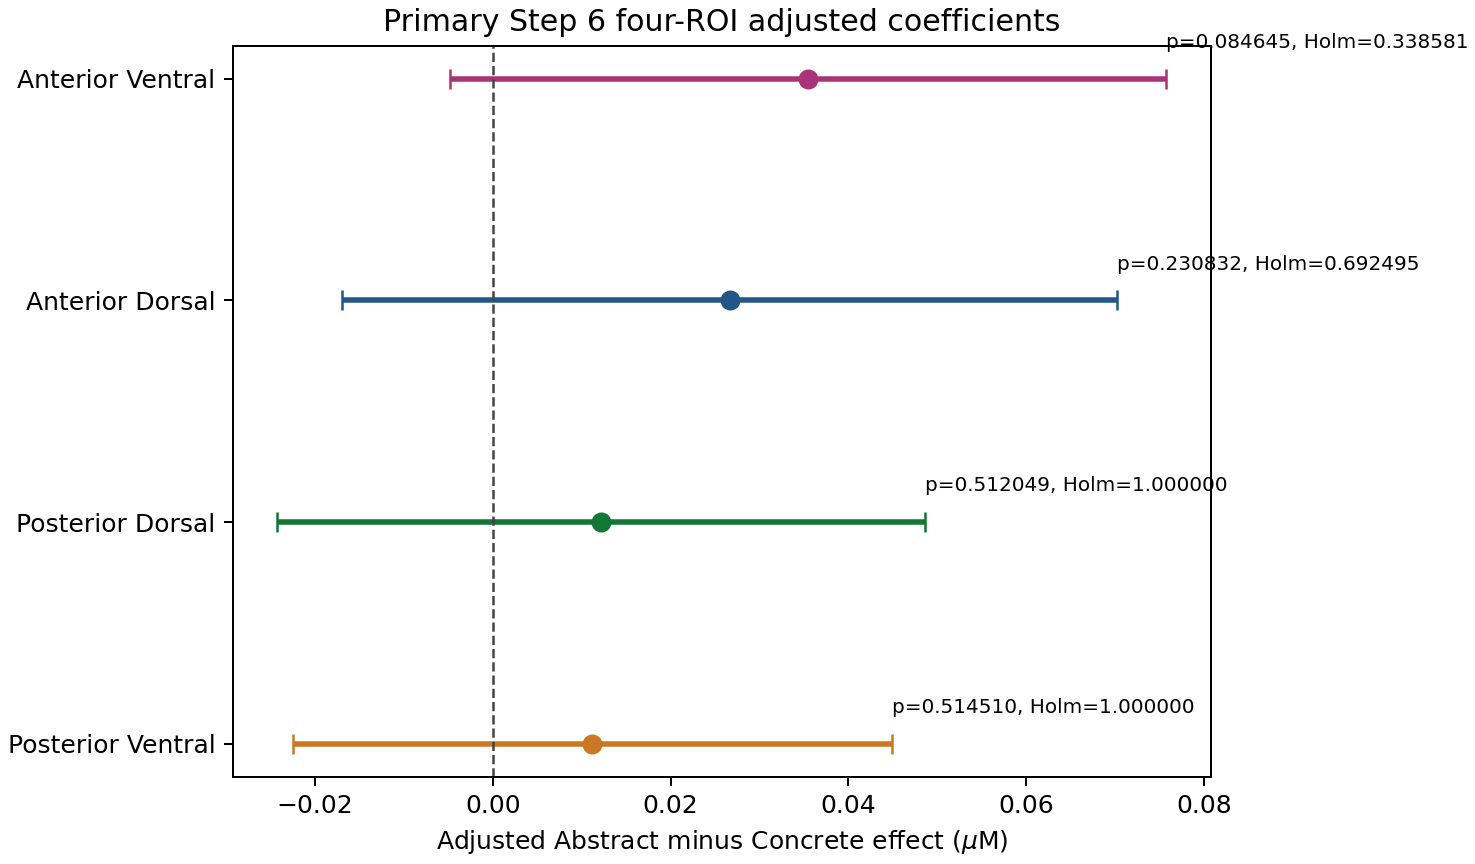
\includegraphics[width=0.92\linewidth]{../visuals/primary_roi_condition_coefficients.png}
\caption{Primary adjusted Abstract-minus-Concrete coefficients for the four revised ROIs, with 95\% confidence intervals and Holm-corrected p-values.}
\end{figure}
\begin{figure}[H]
\centering
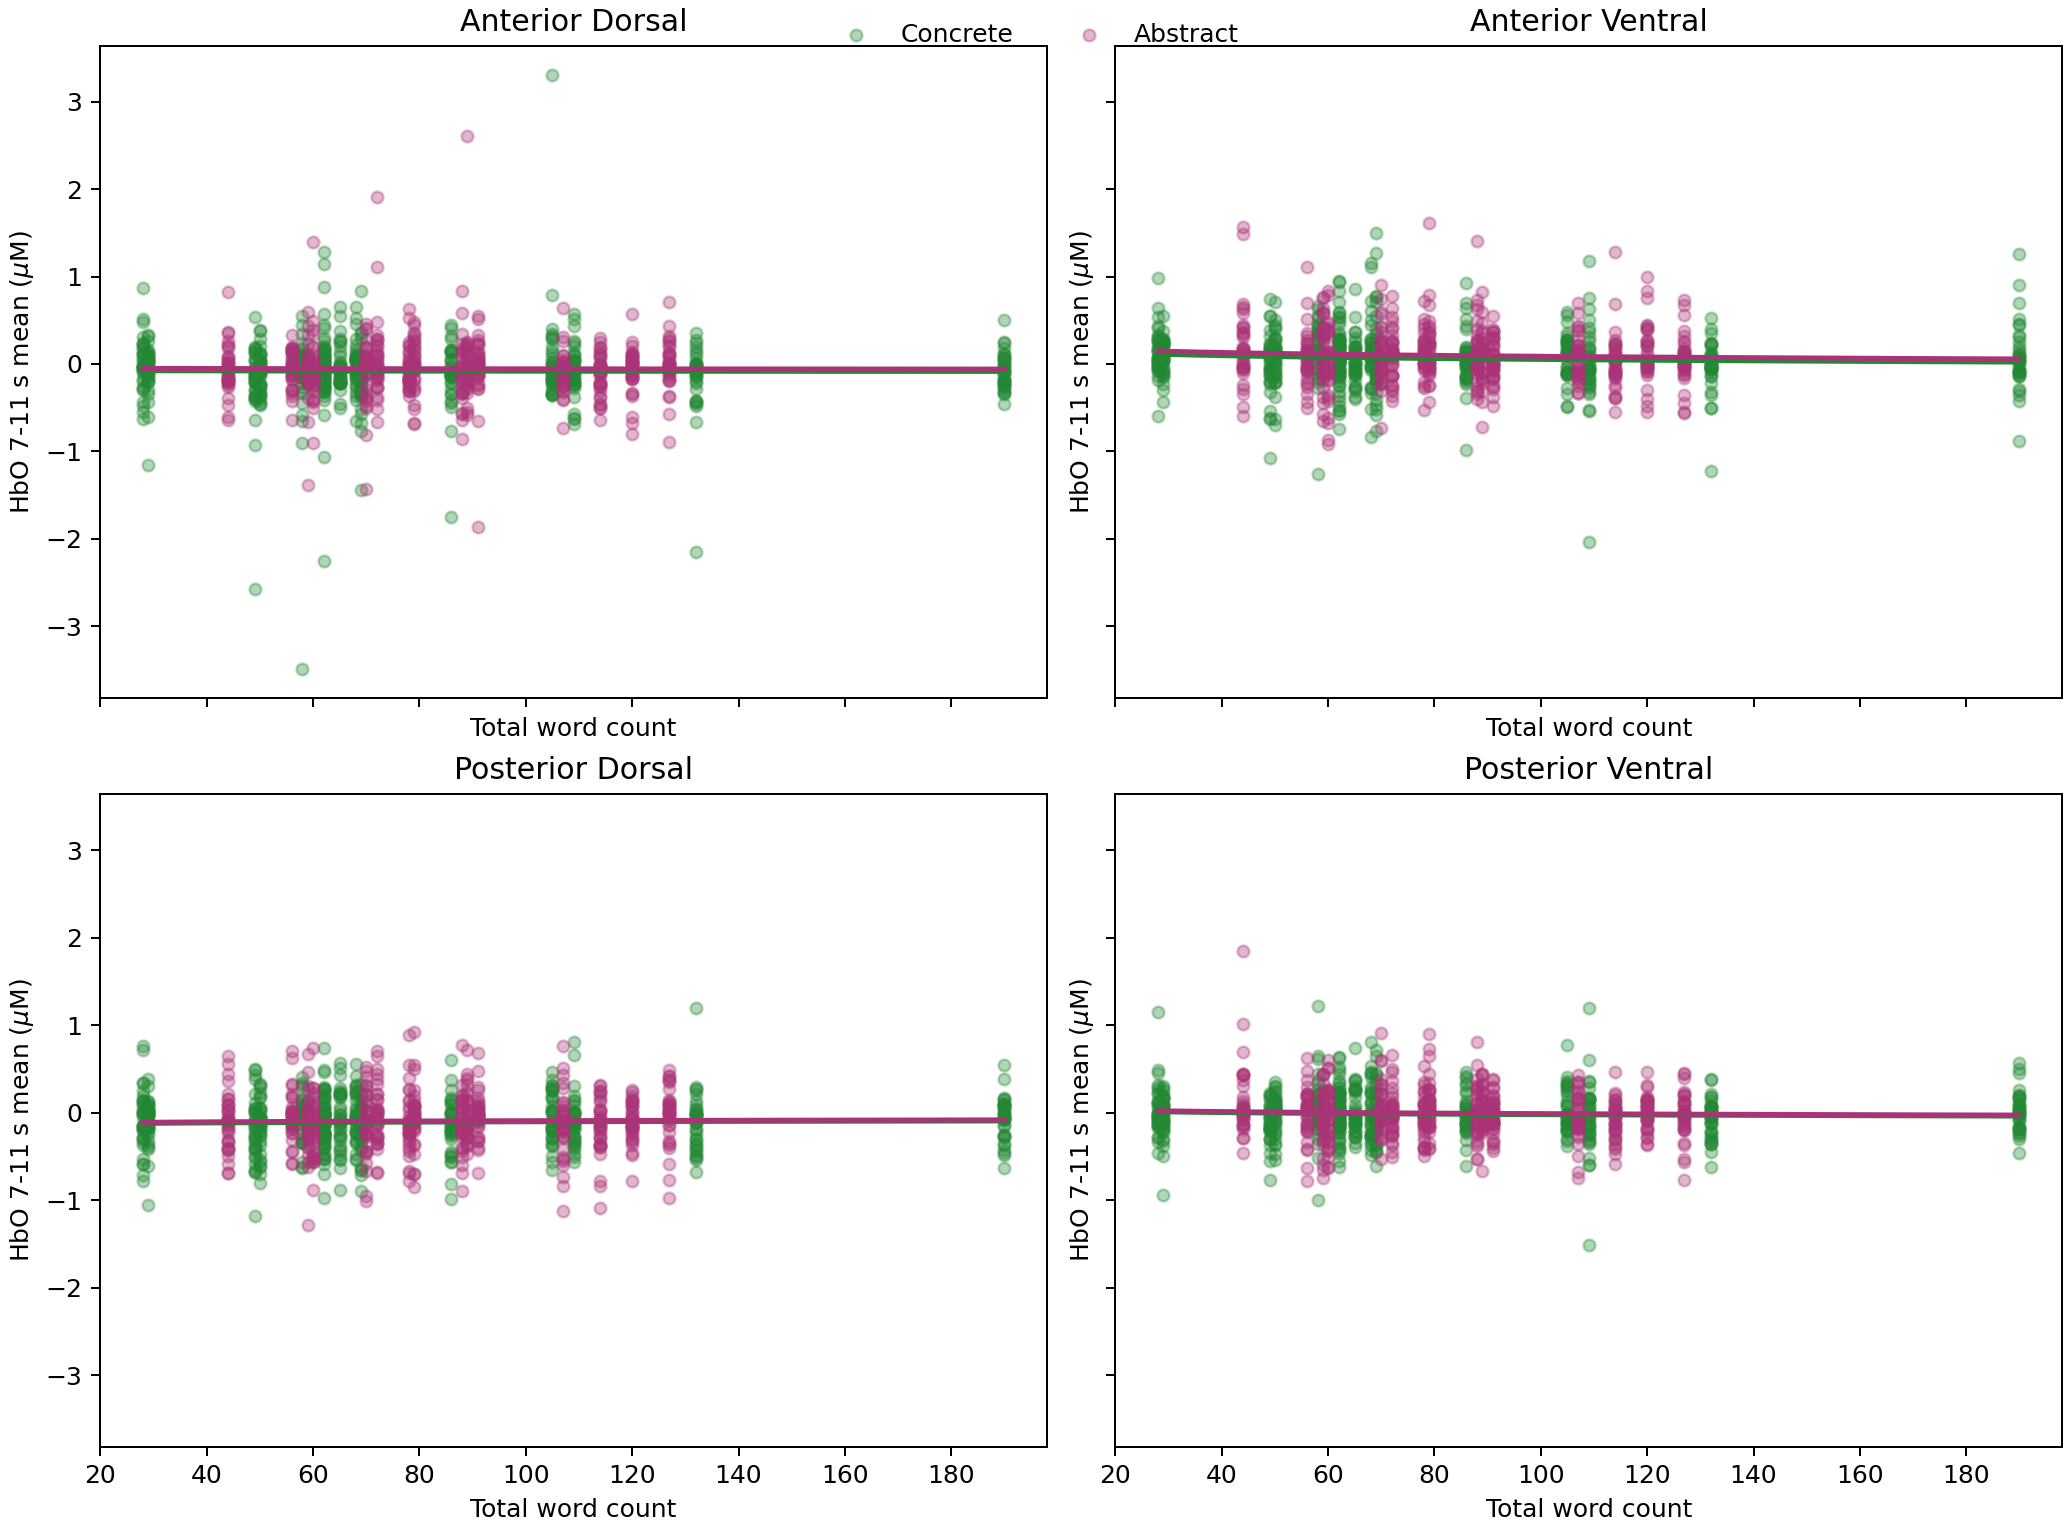
\includegraphics[width=0.48\linewidth]{../visuals/roi_vs_wordcount_scatter_grid.png}
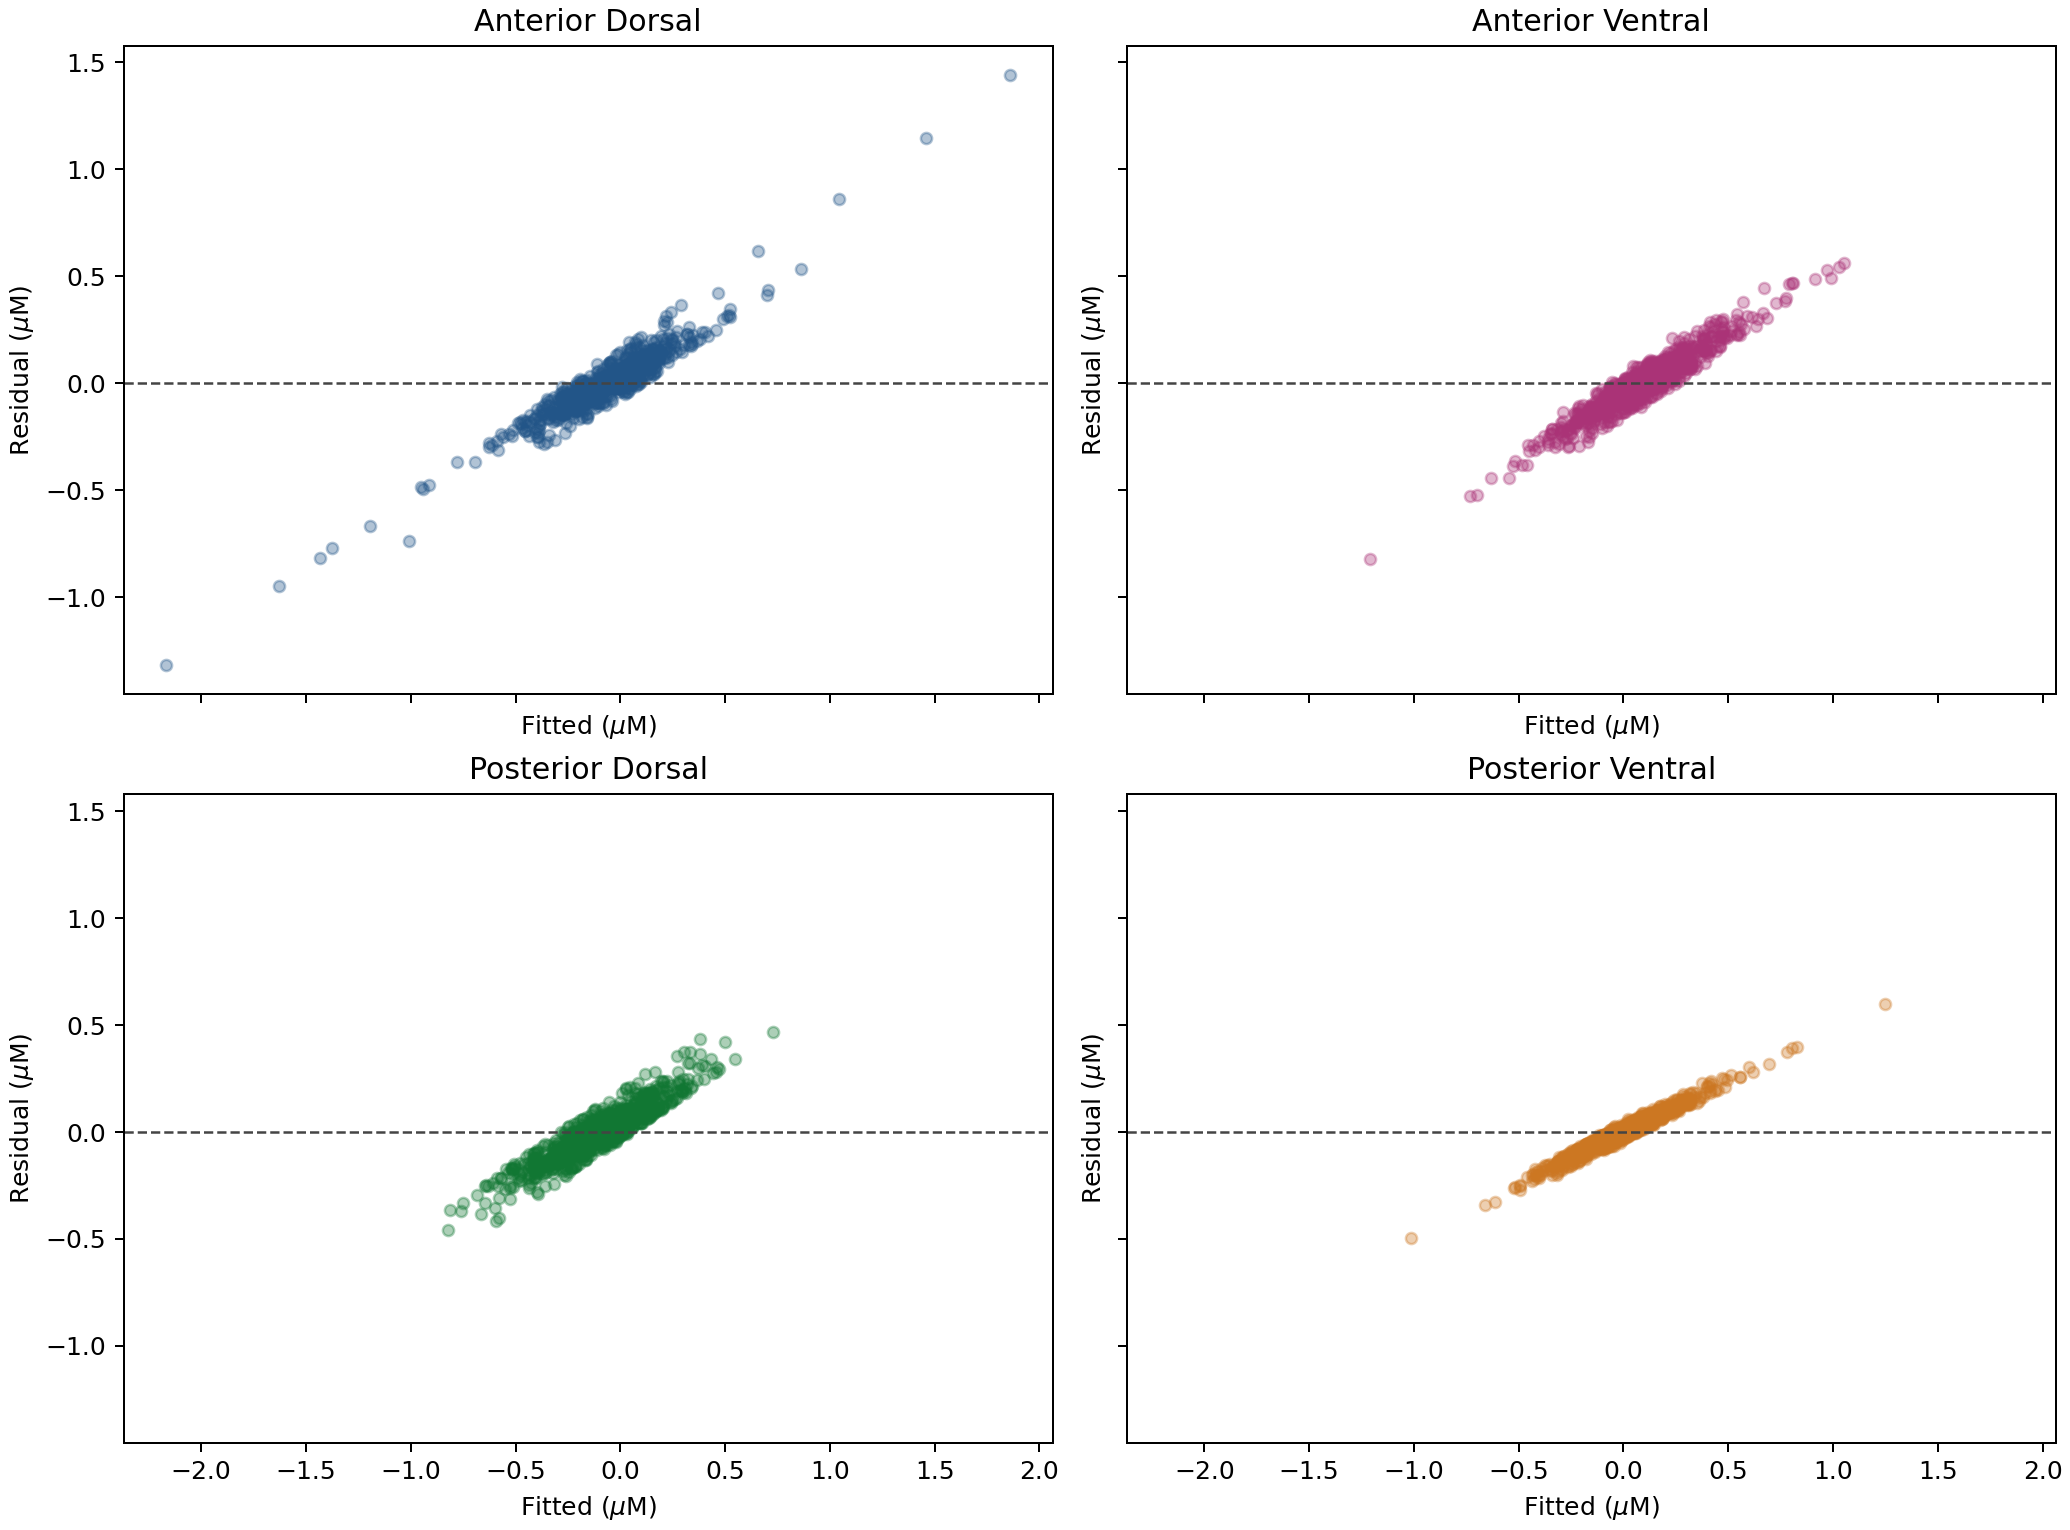
\includegraphics[width=0.48\linewidth]{../visuals/primary_model_residuals_grid.png}
\caption{Primary revised Step~6 ROI-versus-word-count plots and residual diagnostics across the four ROI-specific models.}
\end{figure}
\subsection*{Step 5-Style Supplementary Plots for Step 6}
\begin{figure}[H]
\centering

\includegraphics[width=0.95\linewidth]{../visuals/representative_sensor_geometry.png}
\caption{Representative optode, channel, and source-detector-pair geometry for one Step~6 included participant-session. Blue pairs mark the revised four-ROI analysis montage and short pairs are shown with dashed orange lines.}
\end{figure}
\begin{figure}[H]
\centering

\includegraphics[width=0.48\linewidth]{../visuals/abstract_trial_consistency.png}

\includegraphics[width=0.48\linewidth]{../visuals/concrete_trial_consistency.png}
\caption{Condition-adapted trial-consistency image plots for the Step~6 trial set.}
\end{figure}
\begin{figure}[H]
\centering

\includegraphics[width=0.95\linewidth]{../visuals/channel_consistency_grid.png}
\caption{Grand-average long-channel response images across channels for the Abstract and Concrete conditions.}
\end{figure}
\begin{figure}[H]
\centering

\includegraphics[width=0.92\linewidth]{../visuals/standard_fnirs_compare.png}
\caption{Standard fNIRS waveform comparison across long channels for the Step~6 trial set.}
\end{figure}
\begin{figure}[H]
\centering

\includegraphics[width=0.95\linewidth]{../visuals/abstract_hbo_joint.png}
\caption{Grand-average HbO topography over time for Abstract questions using the revised Step~6 included trial set and restricted to the four-ROI analysis channels.}
\end{figure}
\begin{figure}[H]
\centering

\includegraphics[width=0.95\linewidth]{../visuals/concrete_hbo_joint.png}
\caption{Grand-average HbO topography over time for Concrete questions using the revised Step~6 included trial set and restricted to the four-ROI analysis channels.}
\end{figure}
\begin{figure}[H]
\centering

\includegraphics[width=0.95\linewidth]{../visuals/abstract_minus_concrete_hbo_joint.png}
\caption{Grand-average Abstract-minus-Concrete HbO topography over time.}
\end{figure}
\begin{figure}[H]
\centering

\includegraphics[width=0.48\linewidth]{../visuals/abstract_hbo_topomap_series.png}

\includegraphics[width=0.48\linewidth]{../visuals/concrete_hbo_topomap_series.png}
\caption{HbO topographic time series from 4.0~s to 10.0~s for the Abstract and Concrete conditions.}
\end{figure}
\begin{figure}[H]
\centering

\includegraphics[width=0.48\linewidth]{../visuals/abstract_hbr_topomap_series.png}

\includegraphics[width=0.48\linewidth]{../visuals/concrete_hbr_topomap_series.png}
\caption{HbR topographic time series from 4.0~s to 10.0~s for the Abstract and Concrete conditions.}
\end{figure}
\begin{figure}[H]
\centering

\includegraphics[width=0.95\linewidth]{../visuals/abstract_concrete_single_time_comparison.png}
\caption{Single-time comparison at 9.0~s for Abstract, Concrete, and Abstract-minus-Concrete topographies for both HbO and HbR.}
\end{figure}
\begin{figure}[H]
\centering

\includegraphics[width=0.95\linewidth]{../visuals/abstract_concrete_hbo_evoked_topo.png}
\caption{HbO waveforms by long channel, overlaid for Abstract and Concrete, to show what drives the descriptive topographic differences.}
\end{figure}
\end{document}
